\documentclass[10pt, twocolumn, letterpaper]{article}

\usepackage{times}
\usepackage{graphicx}
\usepackage{amsmath}
\usepackage{amssymb}
\usepackage{booktabs}
\usepackage{hyperref}
\usepackage{geometry}
\geometry{margin=1in}
\usepackage{subcaption}
\usepackage{float}
\usepackage{placeins}
\title{LoRaMAS: Multi-Agent Verification for LoRaWAN Security}
\author{Vayun Gupta \\ University of Illinois Urbana-Champaign \\ Fall 2025 \\ \textbf{Supervisor:} Prof. Klara Nahrstedt, \textbf{Mentor:} Ragini Gupta}


\usepackage{xcolor}

\newcommand{\ragini}[1]{\textcolor{red}{\textbf{[Ragini: #1]}}}
\begin{document}

\maketitle

\begin{abstract}
Internet of Things (IoT) systems increasingly rely on reported sensor locations for critical services including asset tracking, environmental monitoring, and security applications. However, sensors can maliciously spoof their location, and traditional RF-based localization methods remain vulnerable to both adversarial manipulation and environmental distortion. This paper introduces an agentic trust verification framework that transforms localization from a single-shot estimation problem into an iterative, multi-modal reasoning process. Our approach employs specialized agents (RF, Environment, Temporal, and Supervisor agents) that collaboratively verify location claims by calling tools such as trilateration, LOS estimation from satellite imagery, and temporal consistency checks. Unlike black-box classifiers, our framework provides explainable trust decisions and adaptive evidence collection. Using a LoRaWAN dataset from the University of Virginia, pure trilateration achieves a median localization error of 206.99 m and gradient-boosting regression achieves 180.86 m in a challenging urban-indoor environment. On injected verification attacks, LoRaMAS improves attack-detection accuracy from 0.532 for the RF/trilateration baseline to 0.798, improves F1 from 0.672 to 0.881, and reduces false negatives from 0.494 to 0.213 while maintaining zero false positives on the evaluated benchmark. The overhead of agentic verification is acceptable (one supervisor verification round per claim), making this approach practical for real-time IoT applications.
\end{abstract}

\section{Introduction}

IoT systems depend critically on accurate location information from distributed sensors. The increasing adoption of IoT sensors and location-based services has introduced significant security and privacy challenges. These systems are vulnerable to a broad spectrum of attacks that can compromise the integrity, availability, and trustworthiness of sensor-reported information. At the communication level, adversaries may launch denial-of-service (DoS) attacks, packet manipulation, or node misbehavior to disrupt connectivity between sensors and access points. At the sensing level, attackers can inject false sensor readings or manipulate signal characteristics such as RSSI and SNR to falsify localization outcomes. Location-based services are also particularly susceptible to GPS spoofing and location forgery attacks, where malicious devices intentionally misreport their position to gain unauthorized access or disrupt system operations. Furthermore, compromised or malfunctioning hardware can introduce inconsistent measurements that mimic adversarial behavior. Such attacks can severely impact IoT applications including asset tracking, smart city infrastructure, environmental monitoring, and autonomous logistics, making trustworthy and explainable location verification an essential requirement for future wireless sensing systems \cite{gpspoofing}. In this work we focus on sensor based vulnerabilities, specifically involving the false data injection with sensor acting as an adversary to disrupt the localization system.  Existing approaches to sensor localization face fundamental limitations: 1) GPS provides global positioning but remains spoofable with commercial hardware \cite{gpsattack}. 2) RF-based localization using Received Signal Strength Indicator (RSSI) or Signal-to-Noise Ratio (SNR) from access points (APs) is widely adopted but suffers from environmental sensitivity. Factors such as Multipath fading, non-line-of-sight (NLOS) propagation, and varying AP geometries introduce estimation errors that attackers can exploit \cite{lorawanattack}. 

A substantial body of prior work has explored attacks and defenses for wireless localization systems, particularly in GPS and RF-based positioning \cite{lorasecurity}. Existing defenses, however, often rely on complex signal modeling, expensive hardware modifications, or assumptions that do not hold against sophisticated adversaries. For example, several approaches propose adding encryption or authentication mechanisms to civilian GPS signals to prevent spoofing attacks. While effective in principle, these solutions require costly modifications to both satellites and existing GPS receivers, making large-scale deployment impractical. Other works attempt to detect spoofing by collecting advanced physical-layer measurements such as angle-of-arrival, carrier phase, or antenna-array information. These approaches typically depend on specialized hardware, software-defined radios, or enhanced GPS chipsets, limiting their applicability in commodity IoT systems.

To reduce deployment costs, software-based defenses have also been proposed that monitor sudden changes in signal strength, timing, or trajectory consistency to identify spoofing behavior. However, recent studies demonstrate that sophisticated attackers can perform smooth signal takeover attacks, gradually manipulating signal properties to avoid triggering abrupt anomaly detectors. Researchers have further explored cross-validating GPS signals with auxiliary information sources such as WiFi access points, cellular towers, or alternative GNSS systems including Galileo and GLONASS. Nevertheless, these additional information channels can themselves be manipulated or may not provide sufficiently dense coverage for reliable verification, particularly in sparse IoT deployments \cite{shinan}. Similar limitations exist in LoRaWAN and RSSI-based localization systems, where environmental effects such as multipath propagation, NLOS conditions, and varying gateway geometry make it difficult to distinguish between benign localization errors and intentional spoofing attacks \cite{iotdi1}




\textbf{Contributions and Core challenges:} In this work, rather than relying on a single localization algorithm or a fixed verification pipeline, we propose a multi-agent verification framework that performs iterative and explainable trust reasoning across multiple information sources. Our system first constructs a baseline RF localization estimate using RSSI/SNR-based trilateration from trusted LoRaWAN access points. It then employs specialized agents that collaboratively verify the sensor’s claimed location from different perspectives, including RF consistency, environmental context, and temporal behavior. A supervisor agent coordinates these agents, requests additional evidence when needed, and produces a final trust decision indicating whether the reported location should be accepted, rejected, or flagged as suspicious. The core challenge in verifying the location of sensor lies in distinguishing between two phenomena that produce similar RF signatures: (1) legitimate environmental distortion (to dissociate the poor signal conditions from a spoofed attacked), and (2) when malicious location spoofing with aligned manipulated signal properties. An attacker who falsifies location but adjusts transmitted power to match expected RSSI creates ambiguity that single-modality systems cannot resolve.

Our key contributions are:
\begin{itemize}
    \item A novel agent-based architecture for location trust verification that provides explainable decisions through tool calling and iterative reasoning.
 
    \item A sequential verification protocol that adaptively collects evidence, minimizing unnecessary checks while maintaining detection accuracy.
    \item Experimental evaluation on a real LoRaWAN dataset from the University of Virginia \cite{lorawandataset}. 

       % \item Integration of satellite-derived environmental features (buildings, trees) to explain RF anomalies and reduce false positives.

    \item A satellite-backed environmental context pipeline that uses a pretrained Segment Anything Model (SAM ViT-B) \cite{sam} on campus aerial imagery to derive per-link obstruction features for sensor--gateway paths.
    
\end{itemize}

\section{Related Work}

\subsection{Attacks on Location-based Services}

Location-based services and wireless localization systems are vulnerable to a wide range of security attacks that target the integrity, availability, and trustworthiness of sensor-reported location information. One of the most critical threats is \textit{location spoofing}, where an adversary falsifies its reported coordinates or transmits forged wireless signals to appear at a different physical location. \textit{GPS spoofing} attacks manipulate satellite signals to force receivers to compute incorrect positions, while \textit{RSSI/SNR manipulation} attacks alter RF signal characteristics to deceive localization algorithms. Wireless systems are also susceptible to \textit{jamming attacks}, where adversaries intentionally interfere with communication channels to disrupt packet reception and degrade localization accuracy. In \textit{replay attacks}, previously captured legitimate packets are retransmitted to create false temporal or spatial observations. Furthermore, \textit{Denial-of-Service (DoS)} attacks can overwhelm gateways or communication infrastructure, preventing sensors from reliably transmitting localization information. These attacks are particularly dangerous in IoT and LoRaWAN deployments because resource-constrained devices often lack strong physical-layer verification and robust authentication mechanisms. 

In a recent work on GPS spoofing attacks \cite{wisec1}, the adversary manipulate a victim receiver by transmitting counterfeit satellite signals that override legitimate GPS transmissions. In basic spoofing attacks, a single spoofer broadcasts stronger forged GPS signals to force the receiver to lock onto falsified satellite information, thereby misleading the computed location. More advanced attacks perform smooth signal takeover, where spoofed signals are synchronized with authentic GPS signals and gradually overpower them to avoid abrupt anomalies. Recent work further demonstrates distributed multi-antenna spoofing attacks, where multiple synchronized spoofing antennas emulate signals from different satellite directions simultaneously, allowing attackers to evade angle-of-arrival (AoA)-based defenses while steering victim receivers toward falsified locations with high precision.
LoRaWAN remains vulnerable to several physical- and network-layer attacks including replay attacks, bit-flipping, reactive jamming, wormhole attacks, side-channel key extraction, and denial-of-sleep attacks \cite{lorawanattack}. Attackers can manipulate RSSI/SNR metadata, inject malicious packets, or replay delayed packets to disrupt localization, degrade QoS, or exhaust node batteries. Physical-layer attacks are particularly dangerous because they can bypass traditional cryptographic protections while remaining difficult to detect in low-power IoT deployments. Similarly, in \cite{arxiv} the authors develop adversarial spoofing attacks on LoRa RF fingerprinting systems. Attackers generate rogue LoRa signals that statistically mimic legitimate devices using KDE-based signal synthesis, then apply FGSM adversarial perturbations to manipulate I/Q signal features and force deep-learning classifiers to misclassify rogue devices as legitimate transmitters.

\subsection{Existing trustworthy localization and anti-spoofing methods}
Existing GPS spoofing defenses rely on sensor fusion, signal processing, and machine learning–based anomaly detection. Prior approaches combine GPS with IMUs, visual odometry, or neighboring UAV observations to cross-check navigation consistency, while signal-processing techniques analyze physical-layer features such as C/N0, Doppler shift, pseudorange, RSSI, and angle-of-arrival (AoA) anomalies to identify spoofed signals. Recent ML-based methods further classify spoofed versus authentic GPS signals using tree-based models, CNNs, and ensemble learning on multi-channel GPS measurements \cite{gpsecurity}


Shinan et al.  \cite{shinan} propose a lightweight GPS spoofing defense using off-the-shelf GPS chipsets without requiring antenna arrays or specialized hardware. Their approach rotates a partially blocked GPS receiver to estimate the angle-of-arrival (AoA) of satellite signals from signal-strength variations, then compares the observed AoA patterns with expected satellite constellation geometry to detect spoofing attacks.
Existing security techniques for LoRaWAN \cite{lorasecurity} primarily focus on cryptographic protection and network-layer defenses. Current LoRaWAN deployments rely on AES128-based encryption, message integrity codes (MIC), nonces, and session keys to ensure confidentiality and integrity of communications. Several works have proposed stronger cryptographic mechanisms such as AES256, blockchain-based authentication, public-key infrastructures, and physical unclonable functions (PUFs) to improve resilience against attacks including replay attacks, bit-flipping, brute-force attacks, and key compromise. Other studies explore physical-layer security methods using carrier frequency offsets, RSSI fingerprints, or traffic monitoring to identify malicious devices. However, these approaches either require specialized hardware, introduce additional latency and energy overhead, or primarily focus on securing communication channels rather than verifying the trustworthiness of a sensor’s claimed physical location. In contrast, our work focuses on trustworthy localization and location verification, where the challenge lies in distinguishing malicious location spoofing from legitimate RF distortions caused by environmental effects such as multipath fading and NLOS propagation.

The authors in \cite{wisec2} propose a GPS spoofing detection technique that cross-validates GPS-reported positions using signals from the cellular network infrastructure. Their system estimates the device’s approximate location from nearby GSM base stations using received signal strength (RSS) measurements and weighted centroid localization, then compares this estimate against the GPS location. If the deviation between the GPS position and the cellular-network-based estimate exceeds a predefined threshold consistently over time, the system flags the event as a GPS spoofing attack.


\subsection{Multi-agent systems for cybersecurity}

Recent advances have explored the use of large language models (LLMs) and multi-agent systems for cybersecurity tasks such as intrusion detection, vulnerability exploitation, automated rule generation, and network measurement. IDS-Agent \cite{idsagent}introduces one of the first LLM-powered intrusion detection agents for IoT networks, integrating reasoning, memory, external knowledge retrieval, and multiple ML classifiers to improve explainability and zero-day attack detection in IDS workflows. Similarly, GRIDAI \cite{gridAI} proposes a collaborative multi-agent framework for automatically generating and repairing intrusion detection rules for rule-based NIDS systems. By combining LLM reasoning with validation and repair agents, GRIDAI reduces rule redundancy while improving robustness against evolving Web attack variants.

Beyond intrusion detection, several works investigate autonomous offensive and defensive cybersecurity agents. CVE-Bench \cite{cvebench}and SEC-bench \cite{secbench} evaluate the ability of LLM agents to exploit and patch real-world vulnerabilities using sandboxed environments and multi-agent orchestration frameworks. These studies show that while current agents can partially automate exploit generation and vulnerability patching, they still struggle with complex reasoning, reproducibility, and reliable verification. Airavat \cite{airavat} extends agentic reasoning into Internet measurement by coordinating multiple specialized agents for workflow generation, verification, and validation using knowledge graphs and measurement tools. In wireless and autonomous systems, WirelessAgent \cite{wirelessagent} demonstrates how LLM agents can manage intelligent wireless networking tasks such as network slicing through multimodal perception, reasoning, and action modules. SafeCoop \cite{safecoop} further studies adversarial threats in language-driven collaborative autonomous driving and proposes agentic defense mechanisms combining semantic filtering, multi-source consensus, and language-perception consistency checking. Together, these works highlight the growing role of LLM-based agents in cybersecurity and networked systems, while also exposing challenges related to robustness, trustworthiness, explainability, and adversarial resilience.

Traditional multi-agent systems in wireless networking and cybersecurity primarily focus on distributed coordination, consensus mechanisms, trust scoring, collaborative sensing, and anomaly detection. These systems typically rely on rule-based logic, optimization methods, reinforcement learning, or statistical inference to enable cooperation among nodes and access points. Prior work by Liu et al. \cite{trad1,trad2} and related collaborative networking frameworks demonstrate how multiple agents can share observations and coordinate decisions to improve robustness and system efficiency. However, these approaches mainly operate on structured signal or network data and lack higher-level reasoning, memory, retrieval, and explainability capabilities. In contrast, recent LLM-based agentic systems such as IDS-Agent, WirelessAgent, SafeCoop, and Airavat extend traditional multi-agent coordination with reasoning-driven workflows that combine memory, external knowledge retrieval, tool usage, reflection, and explainable decision making. Our work follows this emerging direction by moving beyond simple distributed localization toward collaborative trust verification, where multiple agents jointly reason about the trustworthiness of a sensor’s claimed location using heterogeneous RF and contextual evidence.
\section{Motivations}

The limitations of current localization approaches motivate our multi-modal verification framework. Pure RF trilateration produces location estimates but provides no mechanism to assess their trustworthiness. Even when confidence metrics are attached, these typically reflect geometric dilution of precision rather than the possibility of adversarial manipulation. Consider a sensor claiming to be at location $L$ but whose observed RSSI vector deviates from the expected values. Is this deviation caused by:
\begin{enumerate}
    \item NLOS conditions (a building blocking the direct path to an AP)?
    \item Multipath interference (signal reflecting off surfaces)?
    \item Malicious spoofing (the sensor falsifying its location and/or adjusting transmission power)?
\end{enumerate}

Without environmental context, these explanations are indistinguishable. Our framework addresses this by moving from single-shot localization to trust verification using:
\begin{itemize}
    \item \textbf{Multi-modal verification}: Combining RF evidence with environmental context from satellite imagery and temporal consistency.
    \item \textbf{Iterative reasoning}: Agents propose hypotheses, request specific evidence, and refine trust assessments.
    \item \textbf{Explainable decisions}: Each trust decision is accompanied by a chain of reasoning from participating agents.
\end{itemize}

\section{Background}

\subsection{RF-based Localization}

Trilateration using RSSI/SNR is the predominant approach for indoor and dense urban localization. The fundamental relationship between received power and distance is modeled by the log-distance path loss equation:

\begin{equation}
P_r(d) = P_t + K - 10\eta \log_{10}\left(\frac{d}{d_0}\right) + X_g
\end{equation}

where $P_r$ is received power, $P_t$ is transmit power, $K$ is a system constant, $\eta$ is the path loss exponent, $d_0$ is a reference distance, and $X_g$ represents shadow fading.

Given RSSI measurements from $n$ APs with known positions $(x_i, y_i)$, the sensor's location $(x,y)$ can be estimated by solving:

\begin{equation}
d_i = \sqrt{(x - x_i)^2 + (y - y_i)^2}
\end{equation}
\begin{equation}
\text{RSSI}_i = P_t - 10\eta \log_{10}(d_i) + \text{const}
\end{equation}

In practice, this becomes a least squares minimization:

\begin{equation}
\hat{\theta}_{\text{LS}} = \arg\min_{(x,y)} \sum_{i=1}^n \left( \widehat{\text{RSSI}}_i - \text{RSSI}_i \right)^2
\end{equation}

However, this formulation assumes LOS conditions and treats all AP measurements as equally reliable. In real environments, multipath fading and NLOS propagation introduce systematic biases.

\subsection{Environmental Impact on RF Signals}

SatLoc \cite{sateloc} demonstrated that satellite imagery can predict LOS/NLOS conditions for GPS signals in urban canyons. The same principle applies to terrestrial RF localization: buildings and trees attenuate signals, creating predictable deviations from free-space propagation.

A signal is considered LOS if the direct path between sensor and AP is unobstructed. In NLOS conditions, the received signal strength is attenuated, leading the distance estimator to overestimate true distance. This creates characteristic biases: sensors near buildings appear farther from APs on the opposite side of the structure. It is important to note that these environmental effects are not random since they follow geometric patterns determined by the physical environment. Our framework exploits this predictability to distinguish legitimate NLOS-induced deviations from malicious spoofing.

\subsection{Threat Model}

We define our adversary and assumptions precisely:

\textbf{Adversary Capabilities:}
\begin{itemize}
    \item A sensor may falsify its reported location $L_{\text{claimed}} \neq L_{\text{true}}$.
    \item An adversary can manipulate transmitted signal properties (RSSI, SNR) arbitrarily.
    \item The adversary knows the AP positions and can observe normal RF patterns.
    \item Attacks can be persistent (continuous spoofing) or intermittent (spoofing only during critical periods).
\end{itemize}

\textbf{Adversary Goal:}
Appear at a false location while remaining plausible—i.e., the claimed location should not be trivially rejectable by any single modality.

\textbf{Assumptions:}
\begin{itemize}
    \item Access Points (APs) are trusted and cannot be compromised.
    \item Satellite imagery is reliable and available for the deployment area.
    \item The adversary cannot simultaneously and perfectly emulate all verification modalities (RF, environmental, temporal).
    \item Initial sensor registration or secure bootstrapping establishes a baseline trust anchor.
\end{itemize}

This threat model captures realistic attack scenarios while acknowledging that no real system provides absolute security. Fig. \ref{fig:threatmodel} illustrates our threat model with adversary sensor (LoRa transmitter) surrounded by trustworthy access points (LoRa receivers).  


\begin{figure}[ht]
\centering
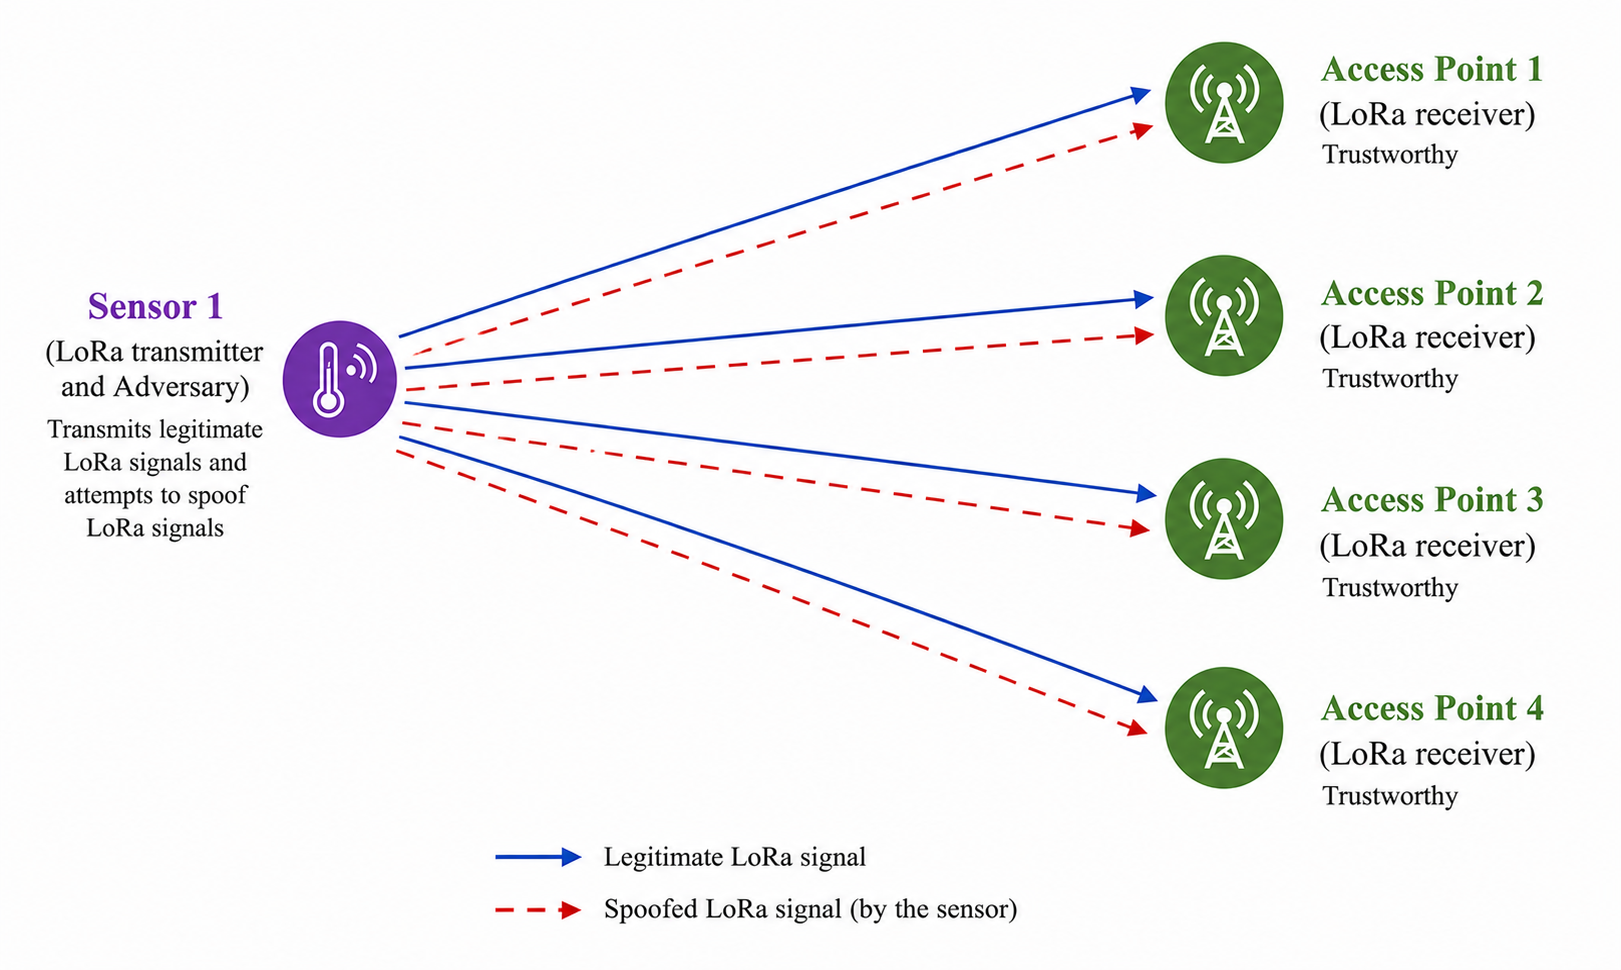
\includegraphics[width=\linewidth]{threatmodel.png}
\caption{Threat Model}
\label{fig:threatmodel}
\end{figure}

\subsection{Multi-Agent Systems for Sensor Verification}

Recent work has explored agent-based approaches for sensor network security. SafeCoop \cite{safecoop} introduced cooperative agents for anomaly detection in industrial IoT, demonstrating that distributed reasoning improves detection of subtle attacks. 

% SPOT \cite{spot} used specialized agents for different attack types, with a coordinator resolving conflicting evidence.

In localization specifically, Liu et al. \cite{trad1,trad2} proposed agent-based collaborative localization where sensors share ranging information and iteratively refine position estimates. However, their focus was on accuracy improvement, not trust verification under adversarial conditions. Our work differs in treating agents as explicit reasoning entities with distinct roles (RF analysis, environmental interpretation, temporal checking) that call tools to gather evidence, a paradigm closer to tool-using language agents than traditional multi-agent systems.

\section{System Design}
Our architecture (Figure \ref{fig:system_diagram}) is implemented as a server-side multi-agent system with four specialized agents:

\textbf{Supervisor Agent}: Orchestrates the verification pipeline, maintains the reasoning state, combines specialist agent outputs, and produces the final trust decision with supporting evidence.

\textbf{RF Agent}: Specializes in signal analysis. It inspects RSSI/SNR shifts, packet-retention ratios, gateway-specific anomalies, and trilateration residuals to quantify RF mismatch.

\textbf{Environment Agent}: Interprets physical context. It uses satellite imagery and a pretrained Segment Anything Model (SAM ViT-B) to derive building/vegetation obstruction features, estimates LOS conditions between each sensor--gateway path, and provides environmental explanations for RF anomalies.

\textbf{Temporal Agent}: Checks consistency across packet history. It analyzes packet witnesses across gateways, replay gaps, delayed duplicates, timestamp skew, and counter regressions to flag replay or timing-based spoofing behavior.

\begin{figure*}[htbp]
    \centering
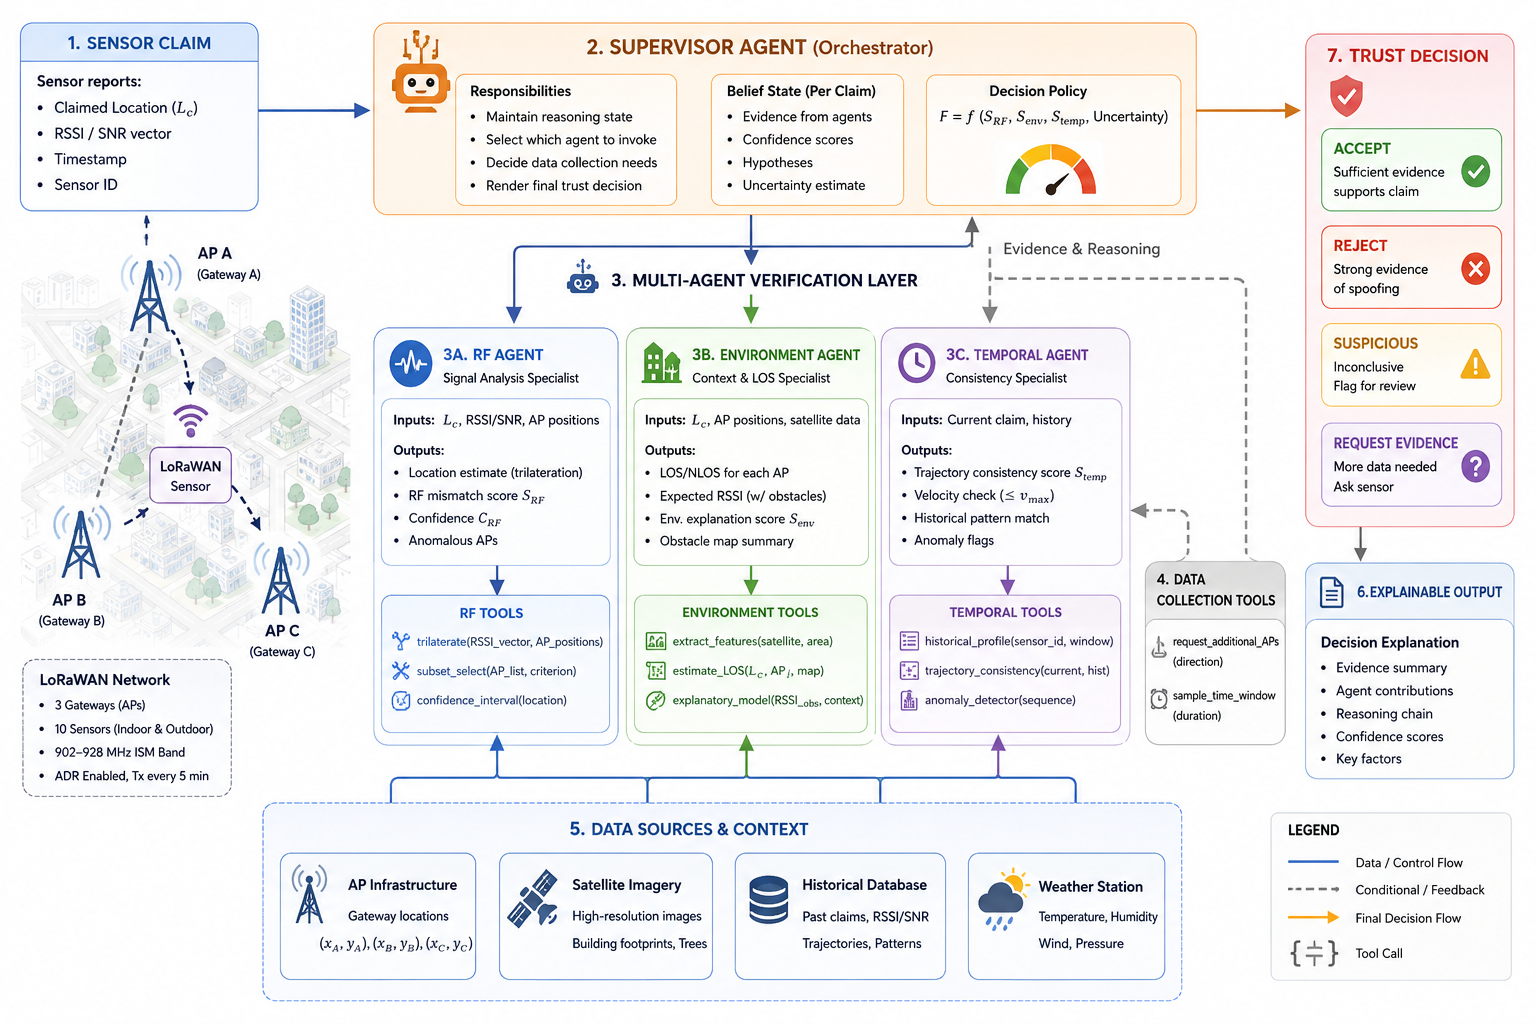
\includegraphics[width=0.82\textwidth]{systemdiagram.png}
    \caption{System architecture showing agent roles and information flow. Sensors report claims to APs. The Supervisor agent orchestrates RF, Environment, and Temporal agents, each calling specialized tools to gather evidence before reaching a trust decision.}
    \label{fig:system_diagram}
\end{figure*}

\subsection{Pipeline Overview}
The LoRaMAS verification pipeline follows a snapshot-to-decision workflow:

\begin{enumerate}
    \item \textbf{Load packet snapshot}: The system loads the current packet observations and compares them against a clean baseline profile of normal RSSI/SNR behavior, packet reception, gateway reliability, and localization residuals.

    \item \textbf{RF analysis}: The RF Agent inspects RSSI/SNR shifts, packet-retention changes, variance changes, and gateway-specific deviations. It also runs trilateration to measure localization error and residual changes.

    \item \textbf{Environmental explanation}: The Environment Agent checks whether RF deviations are physically plausible using satellite-derived context. A pretrained Segment Anything Model (SAM ViT-B) extracts building and vegetation obstruction features for each sensor--gateway path, including LOS blockage, expected extra attenuation, and context fragility.

    \item \textbf{Temporal consistency analysis}: The Temporal Agent analyzes packet-witness consistency across gateways. It checks replay gaps, delayed duplicate packets, timestamp skew, counter regressions, and witness multiplicity.

    \item \textbf{Specialist agent claims}: Each agent produces a claim containing a predicted label, confidence, rationale, and cited evidence keys. These claims summarize whether the anomaly appears sensor-side, gateway-side, temporal, environmental, or benign.

    \item \textbf{Supervisor scoring}: The Supervisor Agent combines structured evidence features and specialist claims using a scoring-based verification rule. Candidate labels include benign, sensor-side manipulation, gateway-side corruption, replay, packet suppression, and counter corruption.

    \item \textbf{Final trust decision}: The supervisor selects the highest-scoring label and outputs an explainable verification report containing the predicted attack type, confidence, suspicious sensor or gateway, cited evidence, and reasoning trace.
\end{enumerate}

\subsection{Baseline: RF-based Localization}

We implement standard trilateration as our baseline. Given $m$ APs with known positions, we solve:

\begin{equation}
\hat{\theta} = \arg\min_{\theta} \sum_{i=1}^m w_i \left( \hat{d}_i - \|\theta - \theta_i\| \right)^2
\end{equation}

where $\hat{d}_i$ is the distance estimated from RSSI using the log-distance model, and $w_i$ are weights (e.g., inverse SNR). The residual error provides an initial confidence metric.

\subsection{Agentic Trust Verification Framework}

\textbf{Motivation for Agents}: Localization is not a one-shot problem. Trust verification requires:
\begin{enumerate}
    \item Iterative reasoning: hypotheses about spoofing must be refined as evidence accumulates
    \item Conflict resolution: RF and environmental evidence may disagree; agents negotiate
    \item Adaptive evidence collection: optimal verification strategies depend on context
\end{enumerate}

Our agent framework treats these requirements as explicit design goals rather than post-hoc additions.


\subsection{Tool Abstraction}

Agents interact with the environment through typed tools implemented in the server:

\textbf{RF Tools:}
\begin{itemize}
    \item \texttt{trilaterate(RSSI\_vector, AP\_positions)}: location estimate and residuals
    \item \texttt{inspect\_sensor(sensor\_id)}: per-gateway RSSI shift, variance shift, packet ratio, and environment context
    \item \texttt{inspect\_gateway(gateway\_id)}: cross-sensor gateway consistency and packet-retention statistics
\end{itemize}

\textbf{Environment Tools:}
\begin{itemize}
    \item \texttt{build\_satellite\_context()}: aerial image, SAM building/vegetation masks, and per-link context CSV
    \item \texttt{inspect\_environment\_context()}: blocked-link fraction, expected extra attenuation, and fragility score
\end{itemize}

\textbf{Temporal Tools:}
\begin{itemize}
    \item \texttt{analyze\_packet\_witness\_consistency()}: replay gaps, delayed duplicates, timestamp skew, and counter regressions
    \item \texttt{lookup\_gateway\_history()}: per-gateway reliability and trust score
\end{itemize}

\textbf{Supervisor Tools:}
\begin{itemize}
    \item \texttt{energy\_graph\_verify()}: explicit label scores over RF, temporal, physical, environment, and availability features
\end{itemize}

\subsubsection{Agent Roles}

\textbf{RF/Gateway Agents}: Produce claims from RSSI and packet-volume evidence. Sensor-side attacks are supported when RSSI shifts concentrate on one sensor across gateways; gateway-side attacks are supported when shifts or packet loss affect many sensors at one gateway.

\textbf{Physical/Environment Agent}: Produces claims from trilateration and satellite-derived path context. A weak link is treated as more plausible when its path crosses vegetation or a SAM-derived hard-obstruction mask, and less plausible when the RF pattern contradicts both distance and environmental context.

\textbf{Temporal Agent}: Produces claims from packet witness evidence. Replay and counter-corruption attacks are supported by delayed duplicates, timestamp skew, replay gaps, and counter regressions.

\textbf{Supervisor Agent}: Combines these claims with calibrated feature templates:

\begin{equation}
Score(y) = \sum_j w_{y,j}x_j + \sum_k \alpha_{y,k}c_k ,
\end{equation}

where $x_j$ are structured evidence features and $c_k$ are specialist-agent claims. The predicted label is the maximum-score label, and confidence is derived from the margin between the top label and the runner-up.

\subsection{Agent Interaction Protocol}

Agents communicate through structured claim objects with the following schema:

\begin{verbatim}
message = {
    "from": agent_id,
    "to": supervisor,
    "role": gateway_local | temporal_consistency | physical_consistency,
    "label": candidate_attack_label,
    "confidence": float,
    "rationale": string,
    "evidence_keys": [string]
}
\end{verbatim}

Key properties:
- \textbf{Explainable}: Each claim includes a human-readable rationale.
- \textbf{Evidence-grounded}: Each claim cites concrete evidence keys from the server.
- \textbf{Ablatable}: Individual roles can be disabled to measure their contribution.

\subsection{Sequential Verification Process}

The supervisor executes this protocol:

\begin{enumerate}
    \item \textbf{Initial RF and packet scan}: Rank suspicious sensors and gateways.
    \item \textbf{Physical check}: Run trilateration and join environment context.
    \item \textbf{Temporal check}: Analyze packet witnesses for replay and counter anomalies.
    \item \textbf{Specialist claims}: Query gateway-local, temporal, and physical roles.
    \item \textbf{Final decision}: Combine evidence and claims with the energy verifier.
\end{enumerate}

\subsection{Decision Policy}

The supervisor outputs one of three verification decisions:

\begin{itemize}
    \item \textbf{Accept}: Sufficient evidence supports claim; localization proceeds.
    \item \textbf{Reject}: Strong evidence of spoofing; claim is discarded.
    \item \textbf{Suspicious}: Inconclusive; claim flagged for human review or secondary verification.
\end{itemize}


\section{Experimental Setup}

\subsection{Testbed Deployment (UVA LoRaWAN Dataset)}

We evaluate our baselines and agentic framework using the real-world LoRaWAN deployment described by Nikseresht et al. \cite{lorawandataset}. Figure \ref{fig:map} shows the deployment map on the University of Virginia campus, covering approximately $590 \times 1120$ meters. 

\begin{figure}[ht]
\centering
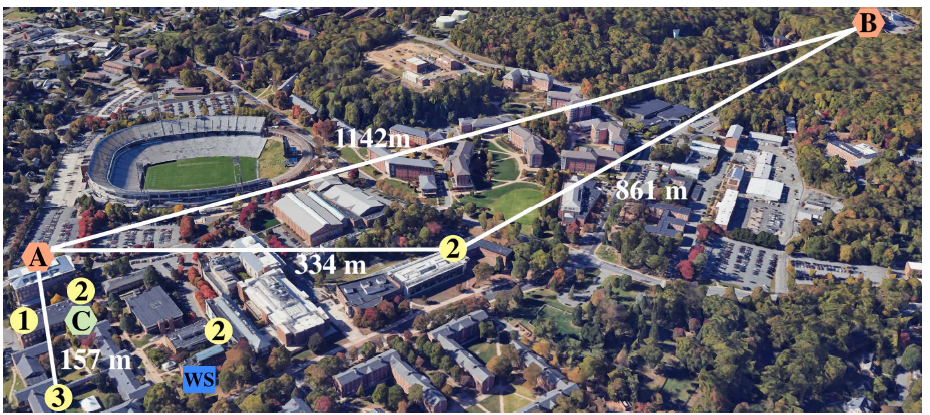
\includegraphics[width=\linewidth]{Dataset.png}
\caption{LoRaWAN Deployment Map (Markers: A, B, C and 1, 2, 3 are Access Points)}
\label{fig:map}
\end{figure}

The infrastructure consists of three gateways (access points):
\begin{itemize}
    \item \textbf{Gateway A (outdoor)}: Mounted on the roof of a five-story office building, providing wide coverage and serving as the primary reference for LOS/NLOS analysis.
    \item \textbf{Gateway B (outdoor)}: Placed on a single-story lab building; experiences longer distances and more obstructions to several sensors.
    \item \textbf{Gateway C (indoor)}: Located on the second floor of a two-story office building beside a window, intentionally introducing NLOS conditions.
\end{itemize}

Ten LoRaWAN sensors (Linovision S500TH and S500CO2) are deployed in four distinct buildings, with pairs of indoor and outdoor sensors. Each sensor transmits every five minutes. The network operates in the 902-928 MHz ISM band with adaptive data rate (ADR) enabled. The dataset includes RSSI, SNR, spreading factor, frequency, bandwidth, airtime, and frame counter for each transmission, collected over 16 months (February 2024 - June 2025). A co-located weather station provides environmental context. The placement of gateways creates diverse propagation conditions: Gateway A has line-of-sight to some sensors (e.g., sensor05, sensor06) and NLOS to others. Gateway C, being indoors, exhibits distinct signal attenuation patterns. This variety makes the dataset ideal for testing trust verification, as RF anomalies can arise from both NLOS obstacles and potential spoofing.

Fig. \ref{fig:dataoflora} represents the original RSSI, SNR, Spreading Factor signal properties along with the corresponding meta-data for communication including the channel bandwidth, transmission frequency, Time of Arrival (ToA) w.r.t each Access Point, receiving Gateway and the Sensor associated for broadcasting. 
\begin{figure}[ht]
\centering
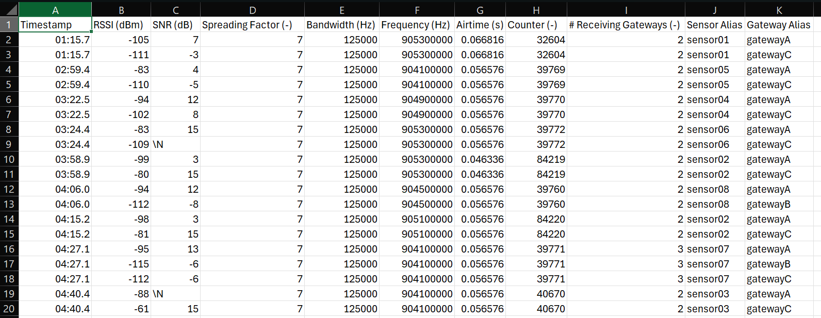
\includegraphics[width=1.1\linewidth]{uvadata.png}
\caption{LoRaWAN dataset}
\label{fig:dataoflora}
\end{figure}


\subsection{Baseline Localization Methods}

We evaluate two baseline localization methods on this dataset:

\begin{enumerate}
    \item \textbf{Pure Trilateration}: Using the log-distance path loss model with a pre-determined forest-like path loss exponent (as the urban environment causes heavy attenuation). RSSI values are converted to distances, and a least-squares solver estimates the sensor position.
    \item \textbf{Regression Model}: We formulate localization as a regression problem, where a gradient boosting regressor learns a mapping from $(RSSI, SNR, gateway\_id)$ to the continuous transmitter distance. The ground-truth distance is computed using the Haversine distance between the sensor and gateway coordinates. Among the evaluated models, gradient boosting achieved the best localization performance and is therefore used in the final system.
\end{enumerate}

\subsection{Attack Scenarios}

We evaluate the verifier with injected attacks over the real UVA packet traces:
\begin{enumerate}
    \item \textbf{Sensor-side RSSI manipulation}: A sensor's received signal profile is shifted or perturbed across gateways.
    \item \textbf{Gateway-side bias}: One gateway reports systematically shifted RSSI values for many sensors.
    \item \textbf{Random RF noise}: Controlled Gaussian perturbations emulate noisy or partially manipulated RF behavior.
    \item \textbf{Availability attacks}: Packet drop and selective suppression reduce gateway observations.
    \item \textbf{Temporal attacks}: Replay, delayed replay, and counter corruption manipulate packet-witness consistency.
\end{enumerate}

\subsection{Metrics}

For baseline localization:

\begin{itemize}
    \item \textbf{CDF of localization error}: Cumulative distribution of Haversine localization errors between estimated and true sensor locations.
    \item \textbf{Median localization error}: The 50th percentile localization error obtained from the CDF curve, representing the typical localization accuracy while being robust to large outlier errors.
\end{itemize}

For agentic evaluation, we report:
\begin{itemize}
    \item overall multi-class accuracy
    \item binary attack-detection accuracy
    \item false positive rate (FPR), false negative rate (FNR), and F1 score
    \item attribution accuracy for attacks with a known corrupted sensor or gateway
    \item mean supervisor verification rounds as the overhead metric
\end{itemize}

\section{Results and Analysis}

\subsection{Path-Loss Modeling Results}

Before evaluating localization performance, we first analyze the relationship between RSSI-derived path loss and transmitter distance under different land-cover environments. Fig. ~\ref{fig:pathloss Vs. Distance} shows the estimated path-loss curves for built-up, forest, field, water, and rangeland environments, together with empirical path-loss measurements derived from the LoRaWAN dataset. As expected, urban built-up regions exhibit the highest attenuation due to dense obstructions and multipath effects, while open environments such as fields and water demonstrate lower propagation loss. These results highlight the strong environmental dependence of RSSI measurements and motivate the need for environment-aware localization and verification methods.

\begin{figure}[t]
    \centering
    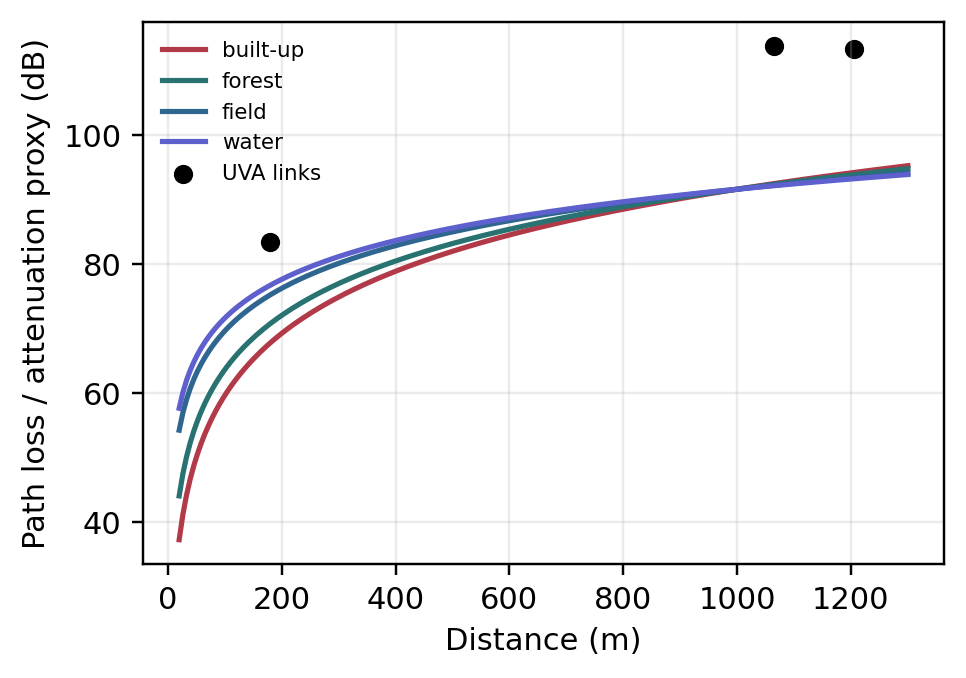
\includegraphics[width=\columnwidth]{pathloss.png}
    \caption{Path-loss versus transmitter distance under different land-cover environments using RSSI-derived propagation models.}
    \label{fig:pathloss Vs. Distance}
\end{figure}


\subsection{Baseline Localization Performance}

Table \ref{tab:baseline} presents the localization error for the two baseline methods on the UVA LoRaWAN dataset. Pure trilateration achieves a median error of 206.99 meters and a 90th percentile error of 304.98 meters. The large errors are due to severe NLOS conditions, multipath fading, and the indoor-outdoor mix in the urban environment.

Regression improves the median error to 180.86 meters and the 90th percentile error to 293.04 meters. By learning from actual (RSSI, SNR, gateway) tuples, the regression model captures some environmental distortions that the theoretical path-loss model misses. Figure~\ref{fig:localization_results} shows the corresponding CDFs.

\begin{figure}[t]
    \centering
    \begin{subfigure}[b]{0.98\columnwidth}
        \centering
        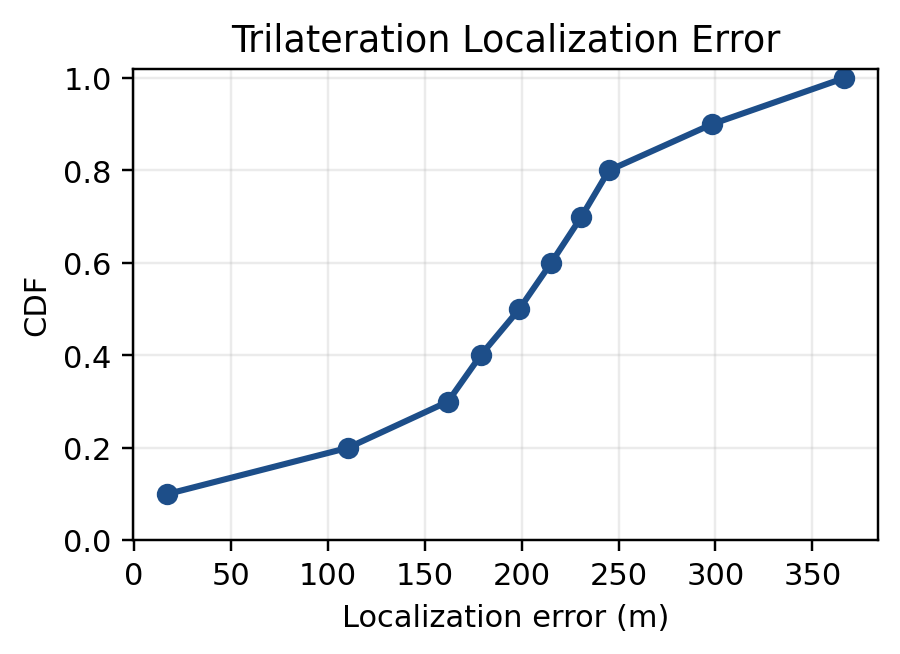
\includegraphics[width=\linewidth]{localization1-trilat.png}
        \caption{CDF of Trilateration based localization errors}
        \label{fig:trilat}
    \end{subfigure}
    \vspace{0.5em}
    \begin{subfigure}[b]{0.98\columnwidth}
        \centering
        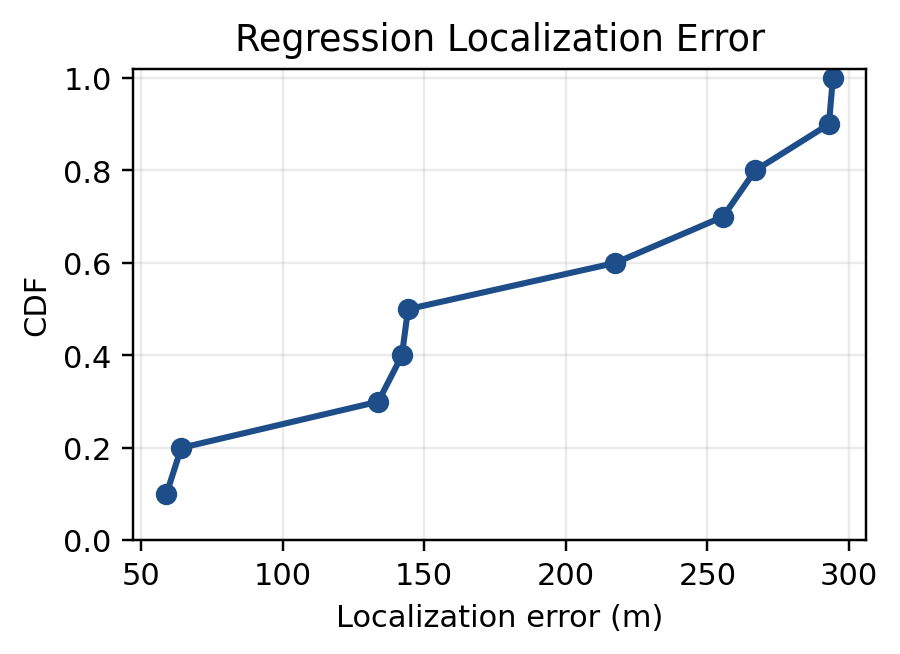
\includegraphics[width=\linewidth]{localization2-regression.png}
        \caption{CDF of Regression based localization errors}
        \label{fig:regression}
    \end{subfigure}
    \caption{Localization performance on the UVA LoRaWAN dataset. (a) Pure trilateration median error: 206.99 m. (b) Gradient boosting regression median error: 180.86 m.}
    \label{fig:localization_results}
\end{figure}

\begin{table}[t]
\centering
\begin{tabular}{lcc}
\toprule
Localization & Median Error (m) & 90th\% Error (m) \\
\midrule
 Trilateration & 206.99 & 304.98\\
 Regression & 180.86 & 293.04 \\
\bottomrule
\end{tabular}
\caption{Localization error of baseline methods on the UVA LoRaWAN dataset. The high errors reflect the challenging urban-indoor environment. The agentic trust verification framework (proposed) aims to detect spoofing rather than directly improve these numbers.}
\label{tab:baseline}
\end{table}

\subsection{Attack Simulation and Localization-Based Detection}

To evaluate robustness against spoofing, we inject adversarial perturbations into the real RSSI observations rather than generating synthetic packets from scratch. The injected scenarios include sensor-side RSSI shifts, gateway-side biases, random RF noise, packet suppression, replay, delayed replay, and counter corruption. These attacks change the evidence seen by the verifier while preserving the underlying UVA packet structure.

Figure~\ref{fig:rssi_snr_spoofing} shows one example for \texttt{sensor05}. The spoof/noise samples are applied on top of each gateway's real RSSI/SNR distribution, so the injected signal remains gateway-specific instead of collapsing into one identical artificial distribution. This matters because the verifier must distinguish true multi-gateway structure from manipulated but still plausible RF observations.

\begin{figure*}[htbp]
    \centering
    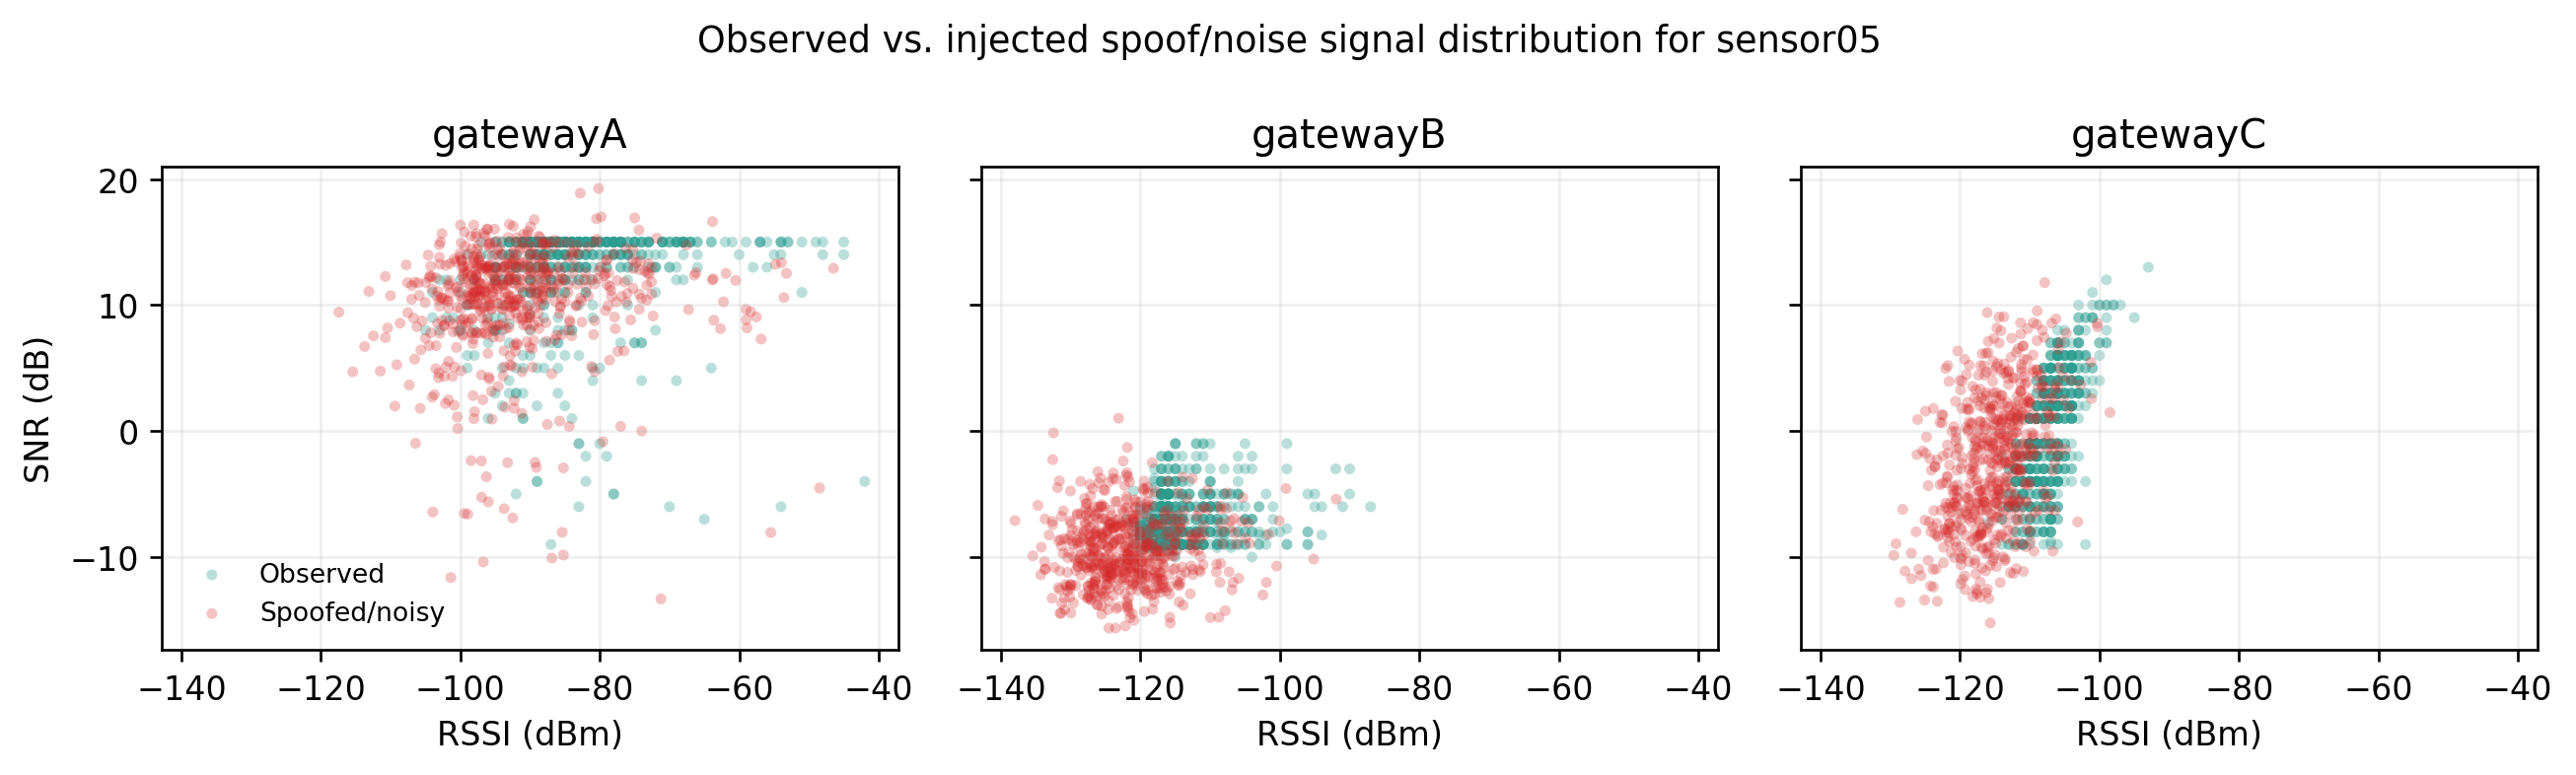
\includegraphics[width=0.82\textwidth]{rssi_snr_spoofing.png}
    \caption{Observed and injected spoof/noise RSSI-SNR distributions for \texttt{sensor05} across the three gateways. The injected samples preserve gateway-specific RF structure because they are sampled around each gateway's real packet distribution.}
    \label{fig:rssi_snr_spoofing}
\end{figure*}

As a simple localization-only detector, we threshold each method's localization error at its clean median error. If an injected scenario produces an error above that threshold, the claim is flagged as suspicious. Table~\ref{tab:localization_detection} reports the resulting detection metrics. The trilateration threshold reaches 0.627 accuracy and 0.705 F1, while the regression threshold reaches only 0.500 accuracy and 0.560 F1. These results show that localization error alone is not reliable enough for trust verification, even when the regression model improves median localization accuracy.

\begin{table}[t]
\centering
\resizebox{\columnwidth}{!}{%
\begin{tabular}{lccccc}
\toprule
Method & Accuracy & FPR & FNR & Precision & F1 \\
\midrule
Trilateration threshold & 0.627 & 0.500 & 0.300 & 0.710 & 0.705\\
Regression threshold & 0.500 & 0.500 & 0.500 & 0.636 & 0.560\\
\bottomrule
\end{tabular}
}
\caption{Spoof-detection performance when localization error is thresholded at each method's clean median error. These baselines show that localization error alone is not sufficient for reliable trust verification.}
\label{tab:localization_detection}
\end{table}

\FloatBarrier

\subsection{Environmental Feature Analysis}

The environmental features explain why localization error alone is a weak trust signal. In the UVA deployment, the same sensor can have one strong gateway link and one weak gateway link because the physical paths are different. For example, \texttt{sensor05--gatewayA} has mean RSSI $-83.36$ dBm and mean SNR $12.83$ dB, while \texttt{sensor05--gatewayB} has mean RSSI $-113.84$ dBm and mean SNR $-7.04$ dB. A pure RF model treats this as a large distance-model mismatch.

The satellite-context tool gives the verifier a physical explanation for this mismatch. It flags \texttt{sensor05--gatewayB} as blocked under the SAM-derived hard-obstruction mask, with building fraction $0.060$, vegetation fraction $0.134$, and expected extra attenuation $3.55$ dB. Therefore, the environment agent does not simply say whether a link is good or bad; it tells the supervisor whether a weak RF observation is plausible under the observed physical context. This helps separate benign NLOS behavior from manipulated RF evidence.

Figure~\ref{fig:satellite_los_overlay} visualizes this satellite-derived context for the deployment area.

\begin{figure}[H]
    \centering
    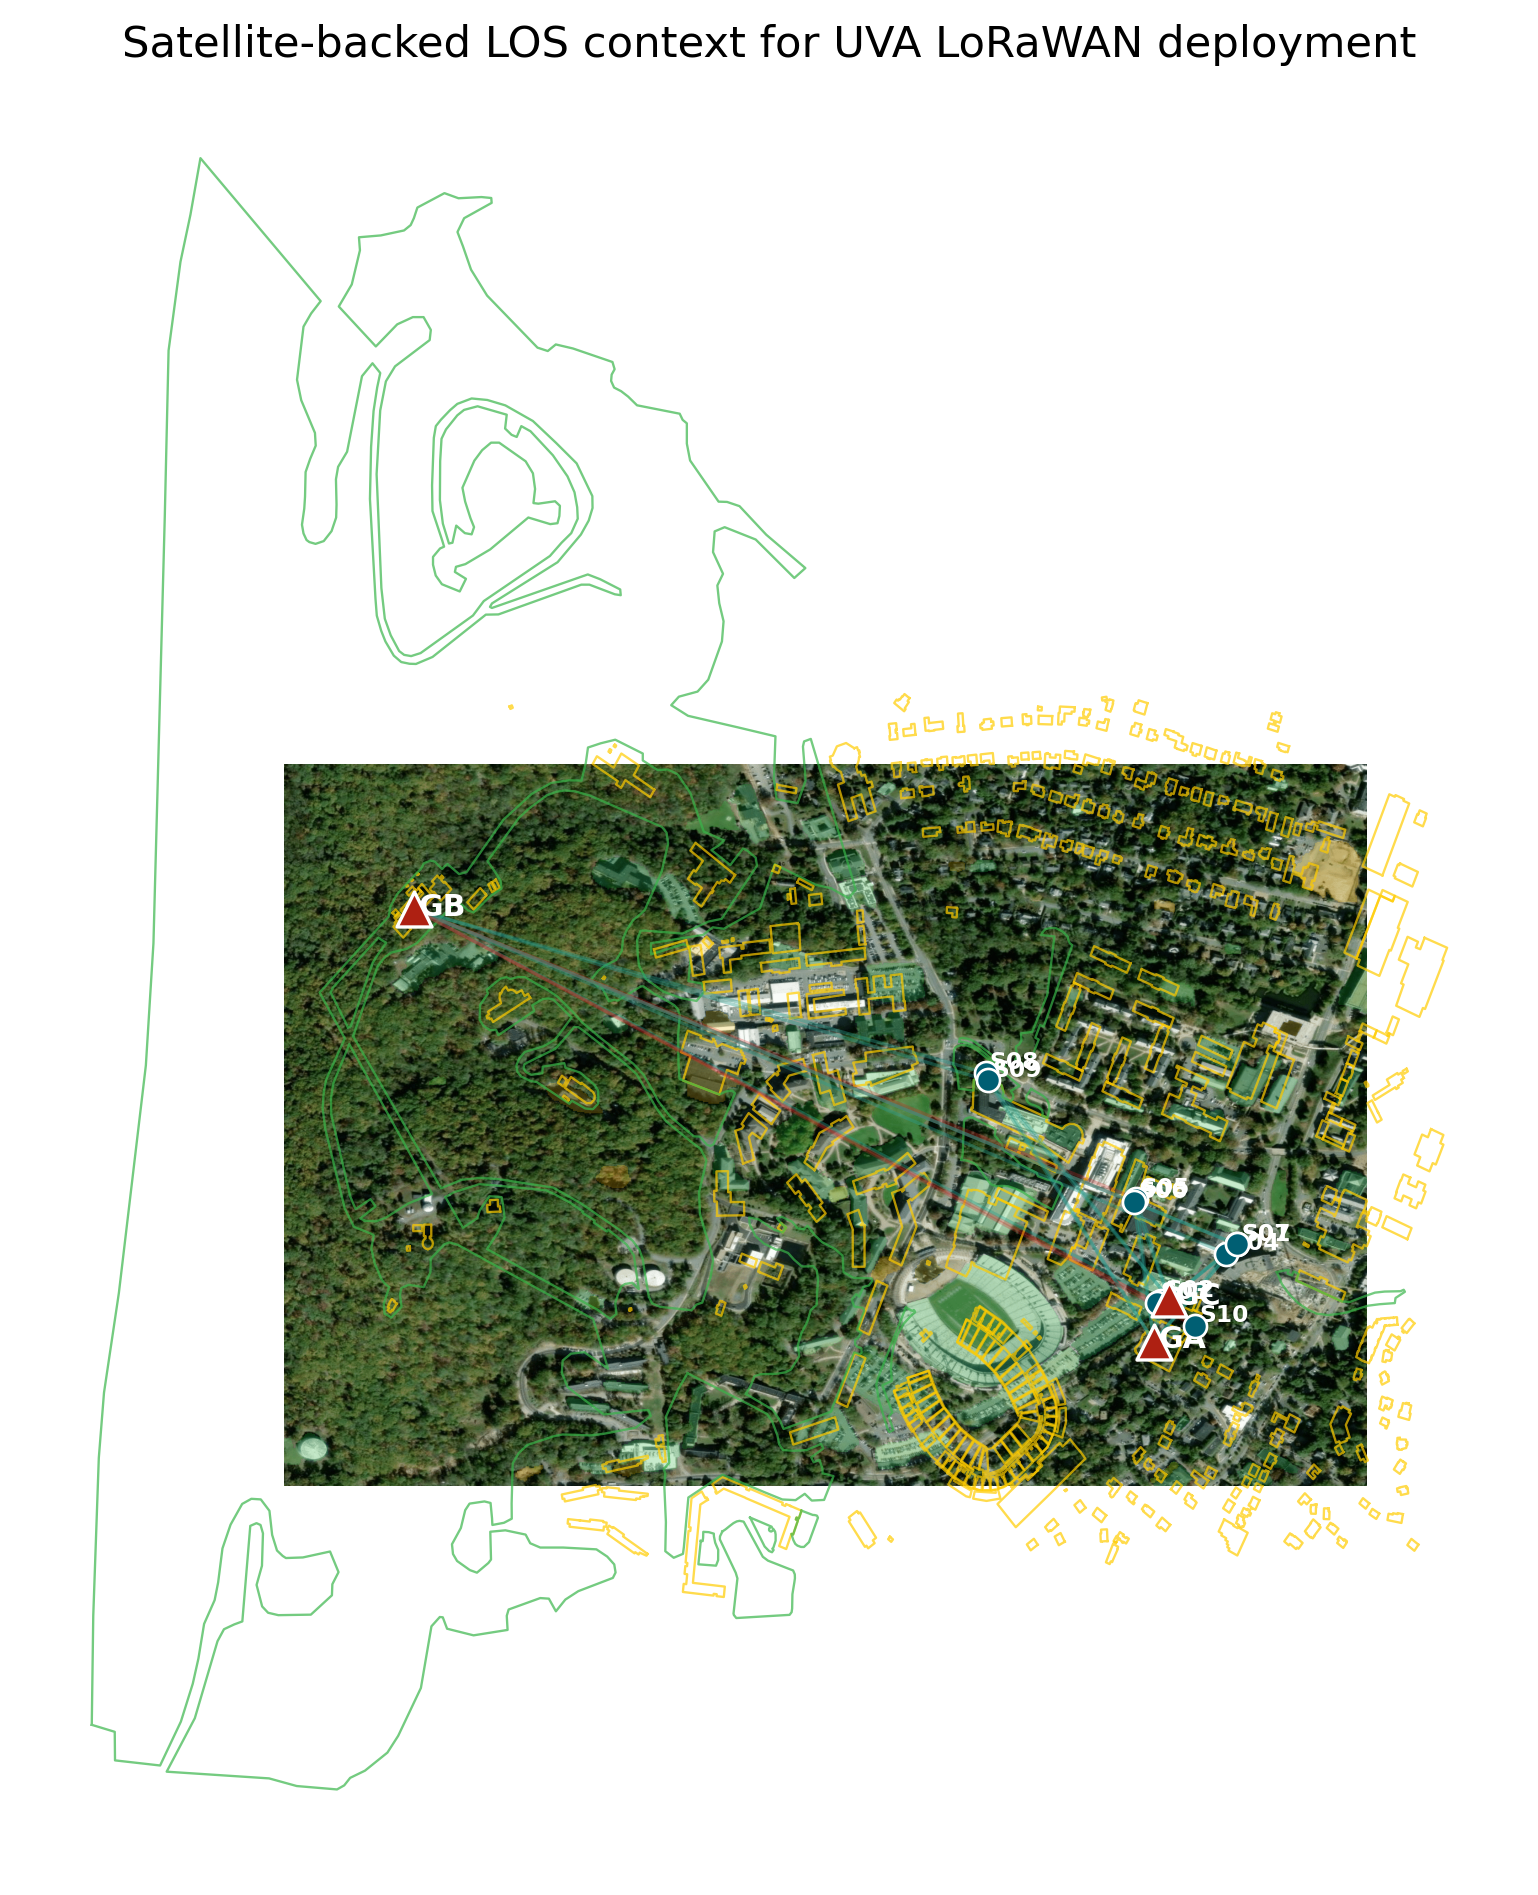
\includegraphics[width=0.95\columnwidth]{satellite_los_overlay.png}
    \caption{Satellite-derived environmental context used by the Environment Agent. The overlay visualizes sensor--gateway paths with LOS/NLOS-style obstruction context from the SAM-derived mask, allowing the verifier to explain weak RF links as physically plausible when paths cross buildings or vegetation.}
    \label{fig:satellite_los_overlay}
\end{figure}

\subsection{Agentic Verification Results}
Table~\ref{tab:mas_results} reports the implemented MAS verification metrics on the injected benchmark. The RF/trilateration baseline has low overall accuracy (0.394) and misses nearly half of the attacks (FNR $=0.494$), showing that RF residuals alone cannot reliably separate spoofing from benign propagation distortion. The centralized trust baseline behaves similarly, with 0.511 attack-detection accuracy and 0.652 F1.

LoRaMAS improves attack-detection accuracy to 0.798 and F1 to 0.881, while reducing FNR from 0.494 to 0.213. The evaluated benchmark has zero false positives for both the RF baseline and LoRaMAS, so the main improvement comes from catching attacks that the RF-only method misses. The ablations show that removing the physical/environment role hurts performance more than removing the temporal role in this benchmark: LoRaMAS-NoPhysical drops to 0.713 overall accuracy and 0.873 F1, while LoRaMAS-NoTemporal matches the full rules model on the current split. This suggests that, for the injected scenarios used here, physical/environment evidence is the more important added modality.

The overhead is small in the current implementation. LoRaMAS uses one supervisor verification round per claim because the RF, physical/environment, and temporal evidence are collected once and then scored by the supervisor. A streaming deployment could cache the clean baseline and satellite context, leaving only packet-snapshot comparison and supervisor scoring on the critical path.

\begin{table*}[ht]
\centering
\begin{tabular}{lcccccc}
\toprule
Method & Overall Acc. & Attack Acc. & FPR & FNR & F1 & Rounds \\
\midrule
RF / Trilateration & 0.394 & 0.532 & 0.000 & 0.494 & 0.672 & 1.0\\
Centralized trust & 0.372 & 0.511 & 0.000 & 0.517 & 0.652 & 1.0\\
LoRaMAS-Rules & 0.777 & 0.798 & 0.000 & 0.213 & 0.881 & 1.0\\
LoRaMAS-NoTemporal & 0.777 & 0.798 & 0.000 & 0.213 & 0.881 & 1.0\\
LoRaMAS-NoPhysical & 0.713 & 0.787 & 0.000 & 0.225 & 0.873 & 1.0\\
\bottomrule
\end{tabular}
\caption{MAS verification results on the injected benchmark. LoRaMAS improves attack detection over RF-only and centralized baselines, primarily by reducing false negatives, with one supervisor verification round per claim in the current implementation.}
\label{tab:mas_results}
\end{table*}

As a representative trace, \texttt{sensor05} has a strong benign link to \texttt{gatewayA} but a much weaker link to \texttt{gatewayB}. The physical/environment agent joins the satellite context and observes that the \texttt{sensor05--gatewayB} path overlaps a SAM-derived obstruction mask. The supervisor can therefore explain the weak gatewayB RSSI as plausible NLOS or partial obstruction instead of treating it as uniformly suspicious. This does not make the link automatically trustworthy; it makes the trust decision evidence-grounded.

\subsection{Discussion}

\subsubsection{When Agents Can Help Most}
Based on the structure of the UVA dataset, we expect agentic verification to provide maximum benefit in:
\begin{itemize}
    \item NLOS configurations (most sensors except sensor05/06)
    \item Periods with variable weather (temperature/humidity affecting RSSI)
    \item Scenarios where an attacker attempts to mimic an NLOS sensor's signal pattern but lacks the correct environmental context.
\end{itemize}

\subsubsection{Expected Failure Modes}
\begin{itemize}
    \item Stale satellite imagery: if a building is constructed after the imagery date, the environment agent may incorrectly attribute spoofing to a nonexistent obstacle.
    \item Very sparse AP deployments (only 2 gateways): trilateration becomes ill-posed, and the RF agent's confidence will be low.
\end{itemize}

\section{Limitations}

Our current work has the following limitations:
\begin{itemize}
    \item \textbf{Injected attacks}: The MAS is evaluated with injected attacks over real traces, not with live adversarial transmissions. The results therefore measure verification behavior under controlled perturbations.
    \item \textbf{Satellite dependence}: Requires up-to-date, high-resolution imagery. The UVA campus is relatively static, but other deployments may change faster.
    \item \textbf{Runtime}: The current offline evaluator loads and compares large packet traces, so benchmark evaluation is slower than a deployed streaming implementation would be.
    \item \textbf{Gateway density}: The UVA deployment has only three gateways; some sensors (e.g., sensor08, sensor09) have intermittent connectivity to gatewayC, reducing the number of usable APs.
\end{itemize}

\section{Future Work}

The most immediate future work is to expand the implemented verifier beyond the current benchmark and test it under live or hardware-in-the-loop attacks. We also plan to:

\begin{itemize}
    \item Integrate weather data (temperature, humidity) as an additional tool for the environment agent, since the UVA dataset includes co-located weather station measurements.
    \item Learn the supervisor's decision policy using reinforcement learning to minimize verification steps while maintaining accuracy.
    \item Explore federated verification: agents running on edge gateways sharing only anonymized trust decisions.
\end{itemize}

\section*{Acknowledgment}

The author thanks Prof. Klara Nahrstedt and Ragini Gupta for their guidance and feedback throughout the independent study.

\section*{Code Availability}

The implementation, experiment scripts, and paper source are available at: \url{https://github.com/Vayung2/LoRaWAN-Agent}.

\bibliographystyle{IEEEtran}
\bibliography{refs}


% \begin{thebibliography}{9}

% \bibitem{satloc} P. Misra, P. Enge, \textit{Global Positioning System: Signals, Measurements, and Performance}, Ganga-Jamuna Press, 2011.

% \bibitem{safecoop} A. Nascimento, et al., ``SafeCoop: Multi-Agent Cooperative Anomaly Detection for Industrial IoT,'' \textit{IEEE IoT Journal}, 2022.

% \bibitem{spot} R. Singh, et al., ``SPOT: Sensor Positioning with Trusted Multi-Agent System,'' \textit{ACM SenSys}, 2021.

% \bibitem{liu2020} Y. Liu, et al., ``Agent-Based Collaborative Localization for Wireless Sensor Networks,'' \textit{IEEE Trans. Mobile Computing}, vol. 19, no. 8, 2020.

% \bibitem{vtdata} University of Virginia, ``LoRaWAN RSSI/SNR Dataset for Urban IoT Localization,'' 2023. Available at [URL].

% \bibitem{halder2021} S. Halder, A. Ghosal, ``A Survey on Mobile Anchor Node Assisted Localization in WSNs,'' \textit{Ad Hoc Networks}, vol. 112, 2021.

% \bibitem{patwari2005} N. Patwari, et al., ``Location Estimation in Sensor Networks,'' \textit{IEEE Signal Processing Magazine}, vol. 22, no. 4, 2005.

% \bibitem{chen2020} J. Chen, et al., ``Secure Localization in the Presence of Byzantine Attacks,'' \textit{IEEE TIFS}, vol. 15, 2020.

% \bibitem{wu2023} L. Wu, et al., ``Multi-Agent Reinforcement Learning for IoT Security,'' \textit{ACM CCS}, 2023.

% \bibitem{zhang2022} K. Zhang, et al., ``Environmental Context for Indoor Localization: A Survey,'' \textit{ACM Computing Surveys}, vol. 54, no. 7, 2022.

% \bibitem{sam}A. Kirillov, E. Mintun, N. Ravi, H. Mao, C. Rolland, L. Gustafson,T. Xiao, S. Whitehead, A. C. Berg, W.-Y. Lo, P. Dollár, and R. Girshick,``Segment Anything,''textit{arXiv preprint arXiv:2304.02643}, 2023.

% \end{thebibliography}

\end{document}
